%!TEX root = ./template-skripsi.tex
%-------------------------------------------------------------------------------
%                            	BAB IV
%               		KESIMPULAN DAN SARAN
%-------------------------------------------------------------------------------

\chapter{HASIL DAN PEMBAHASAN}

\section{Implementasi}
Berikut ini adalah keterangan \emph{flowchart} terkait tahapan penelitian yang sudah berhasil dibuat. Penyempurnaan dari \emph{flowchart} pada Gambar 3.1.

\begin{figure}[H]
  \centering{}
	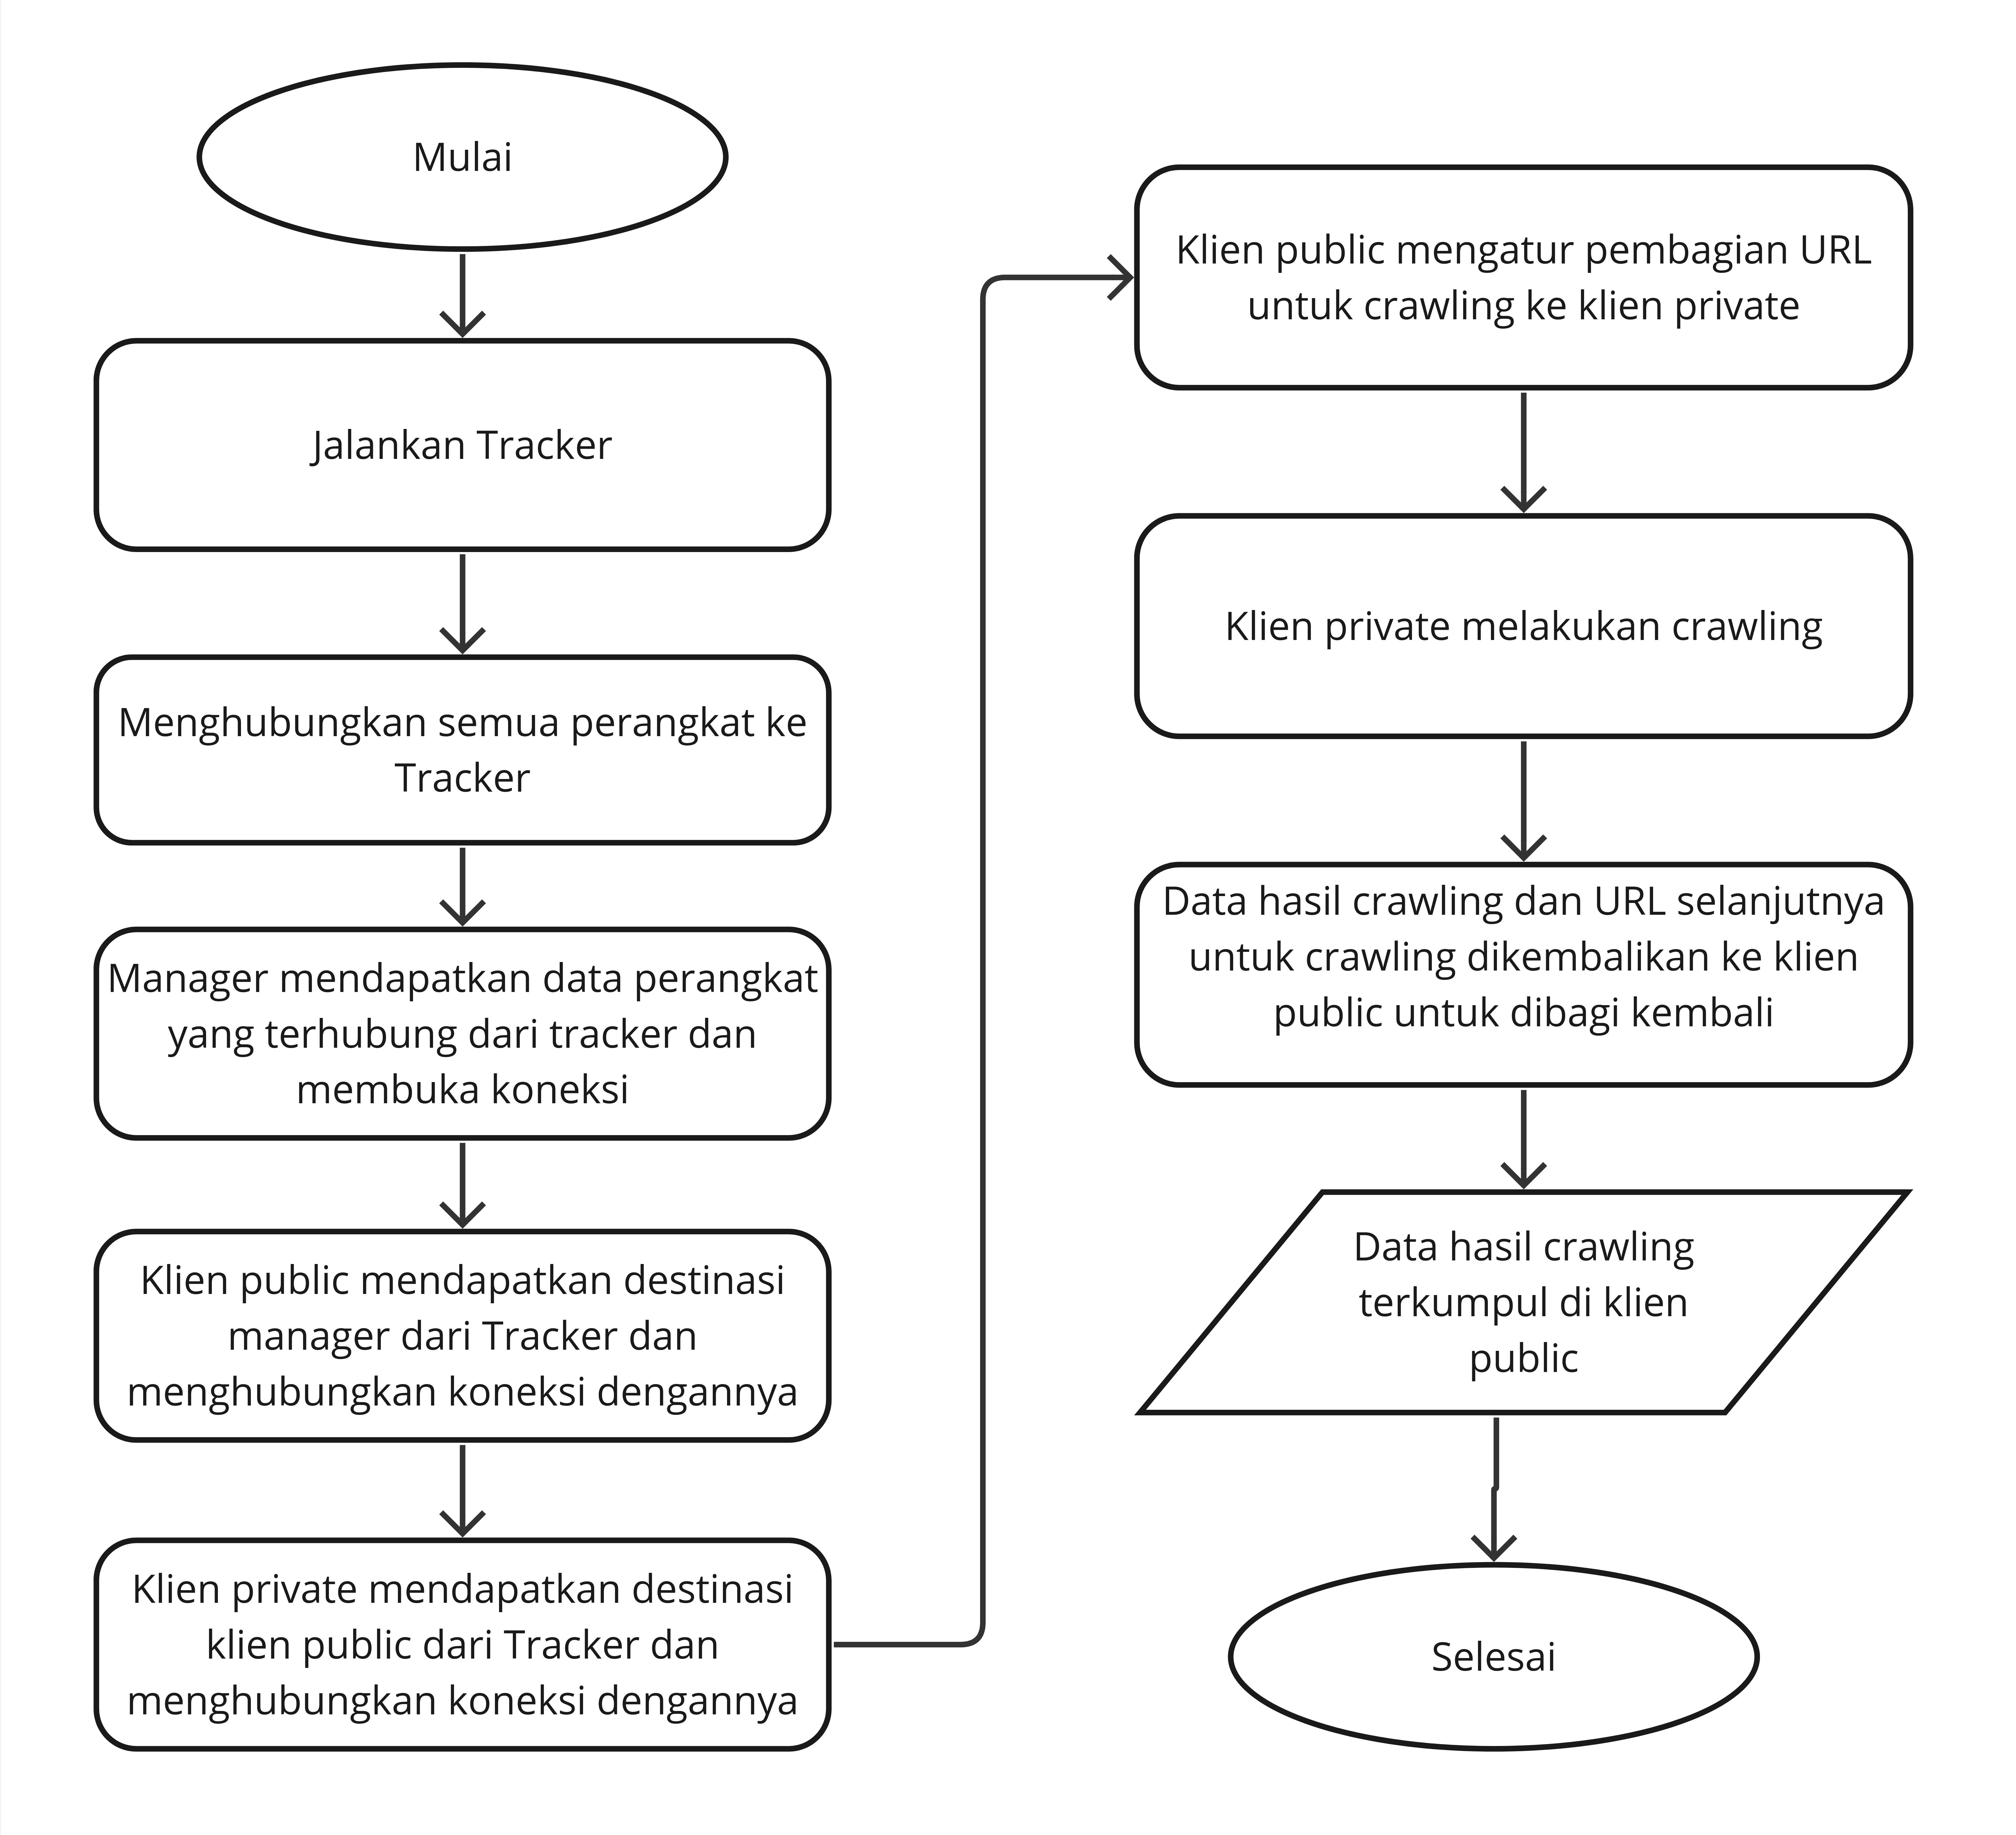
\includegraphics[width=1\textwidth]{gambar/flowchart_crawler_terdistribusi}
  \caption{\emph{Flowchart} Tahapan Penelitian yang Berhasil Dibuat}
\end{figure}

Arsitektur \emph{crawler} terdistribusi dalam penelitian ini terdiri dari lima perangkat lunak dengan konfigurasi tiga perangkat memiliki \emph{public IP address} dan dua perangkat memiliki \emph{private IP address}. Dengan pembagian perannya masing - masing, satu \emph{Tracker}, satu \emph{Manager}, dan tiga Klien. Pada penerapannya setiap program berjalan dengan bahasa pemrograman Python dan setiap proses dapat berjalan secara paralel dengan menggunakan \emph{threading}. Arsitektur ini telah mengalami modifikasi dari yang sebelumnya pada Gambar 3.2. Setelah melakukan percobaan untuk mendapatkan kondisi \emph{peer to peer}, maka dihasilkan arsitektur seperti Gambar 4.2.

\begin{figure}[H]
  \centering{}
	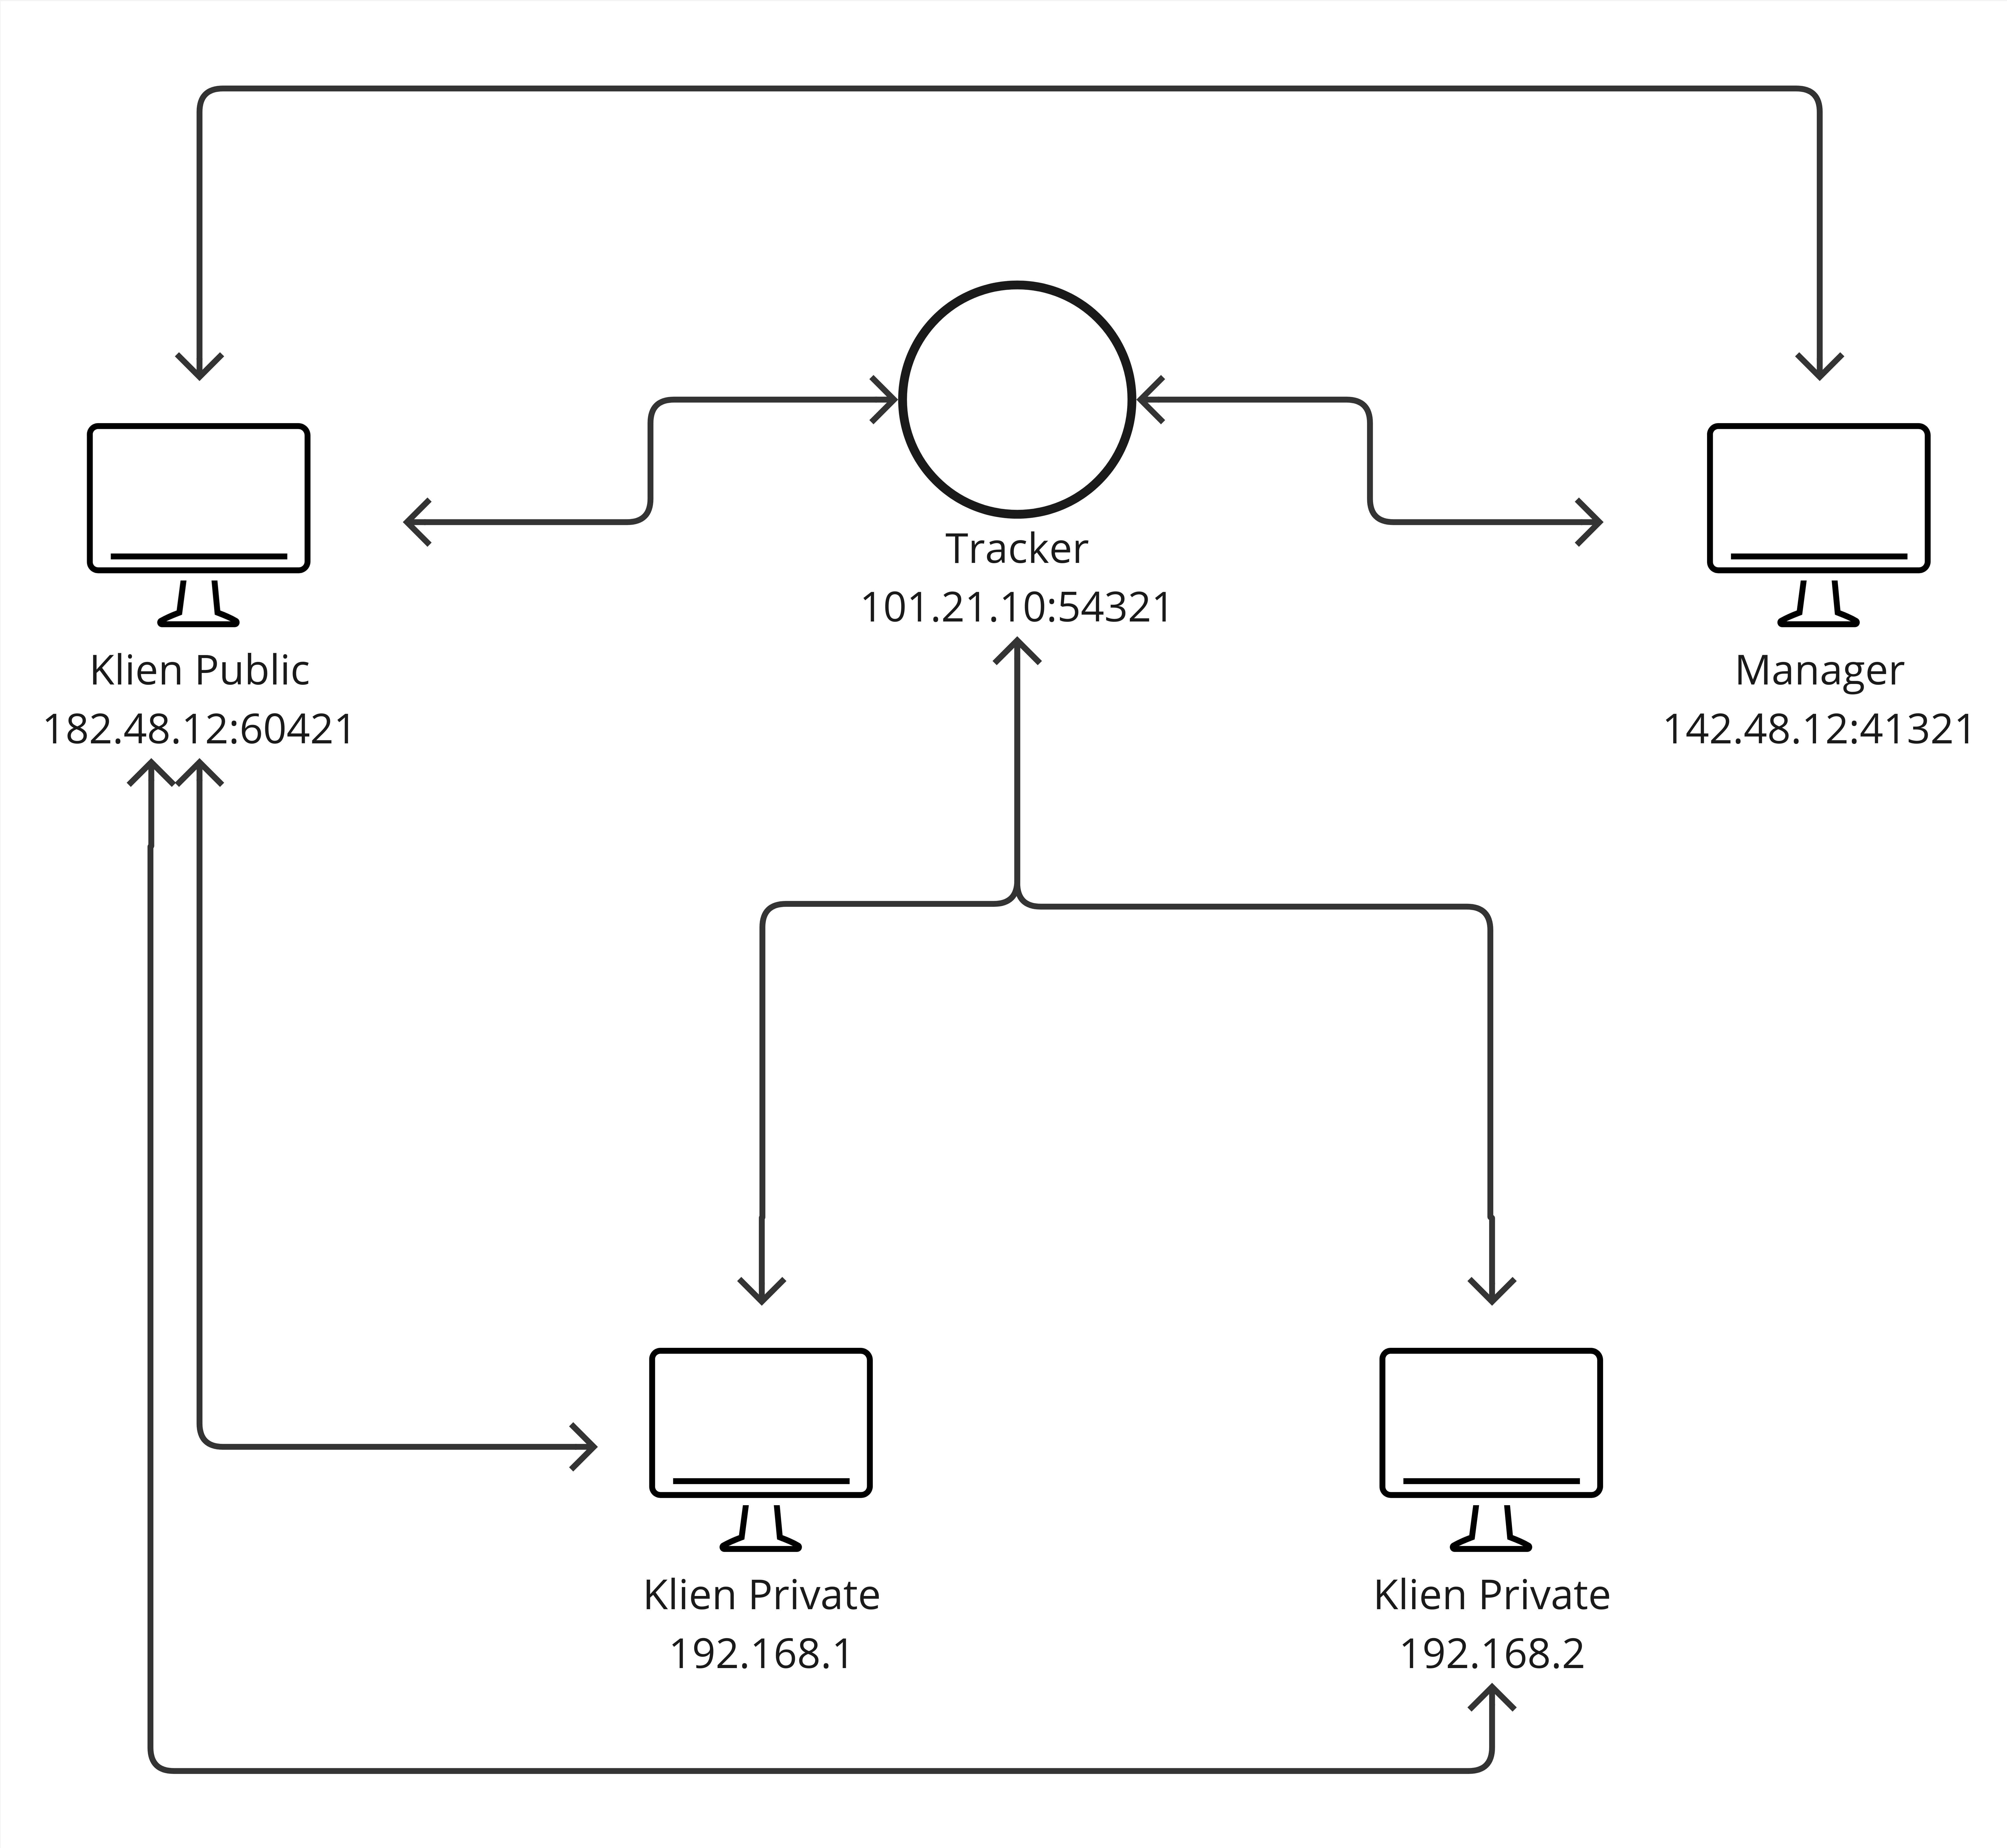
\includegraphics[width=0.6\textwidth]{gambar/arsitektur_baru}
  \caption{Arsitektur \emph{Crawler Terdistribusi}}
\end{figure}

\subsection{\emph{Tracker}}
\emph{Tracker} akan memiliki \emph{public IP address}, dikarenakan \emph{tracker} memiliki tugas sebagai jalur informasi antara perangkat yang terhubung. Setiap perangkat harus terlebih dahulu untuk terhubung melalui \emph{tracker} dan juga mengirimkan informasi apakah perangkat tersebut memiliki \emph{public IP address} atau tidak dan tipe dari perangkat tersebut, apakah dia \emph{manager} atau klien. Lalu, \emph{tracker} akan menampung semua perangkat yang terhubung. 
\clearpage

\begin{figure}[H]
	\centering{}
	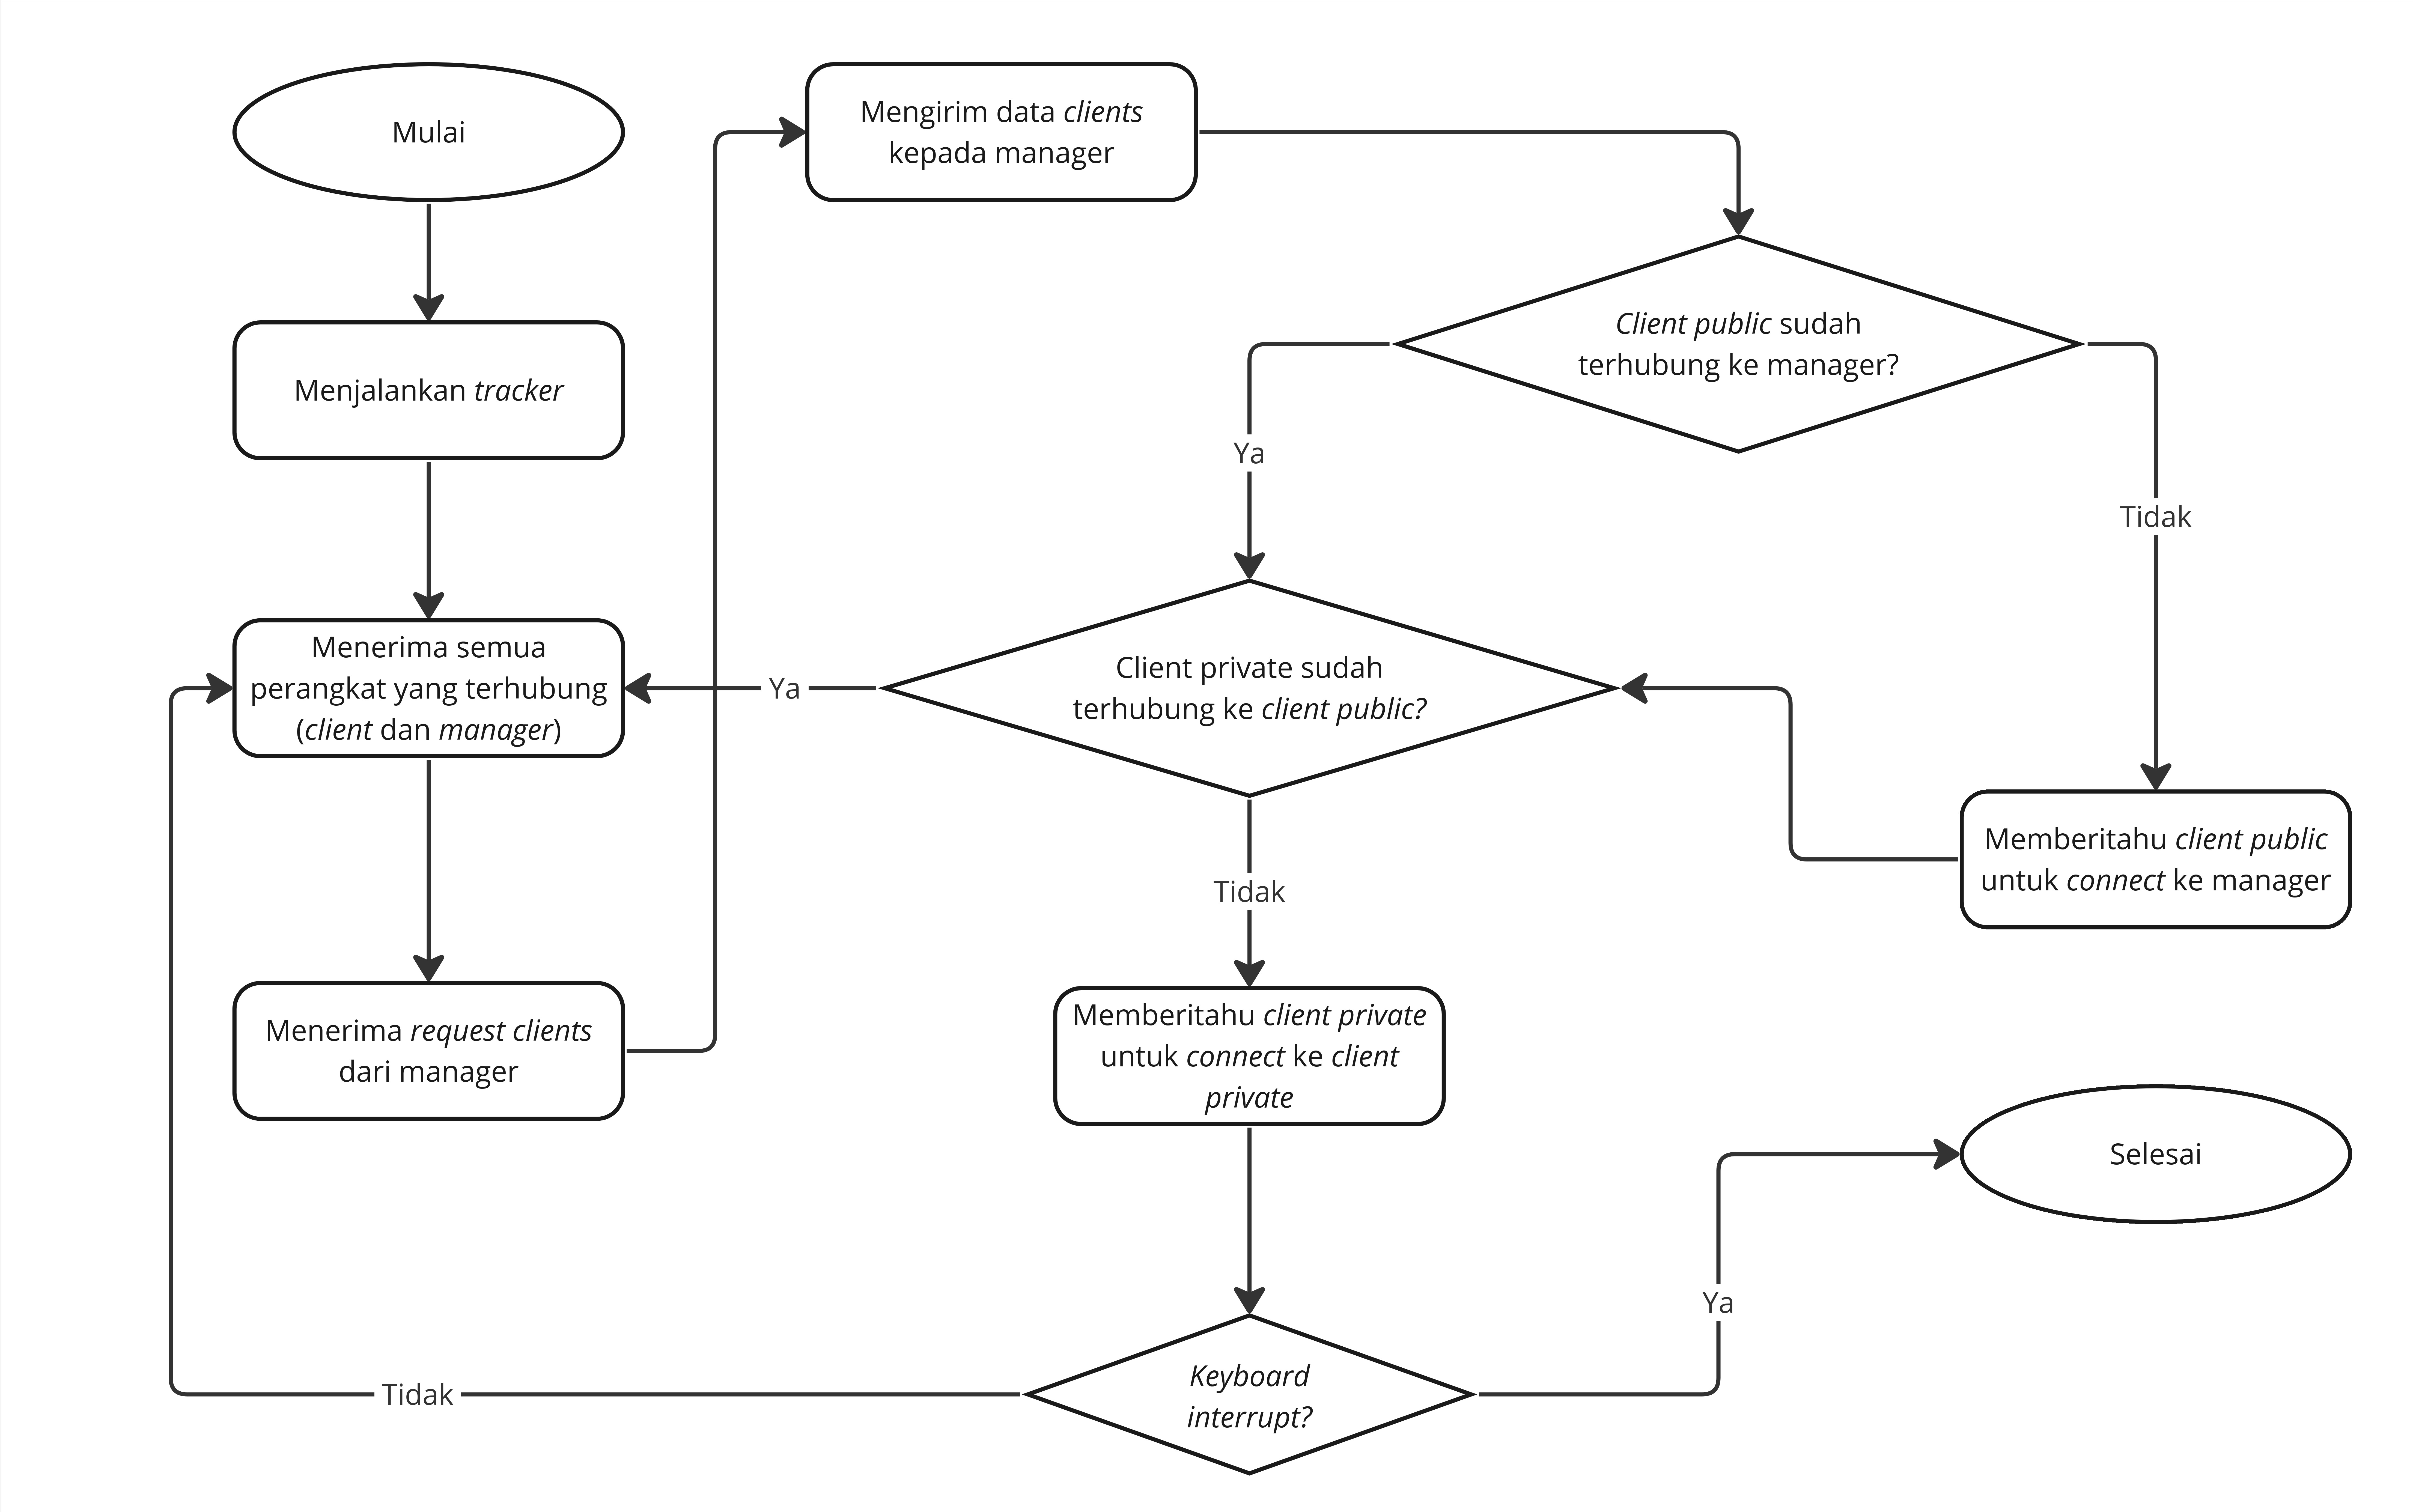
\includegraphics[width=1\textwidth]{gambar/flowchart_tracker}
	\caption{\emph{Flowchart tracker} }
\end{figure}

\begin{itemize}
	\item{Potongan kode untuk mengatur perangkat atau klien yang baru terhubung}
	\begin{figure}[H]
		\centering{}
		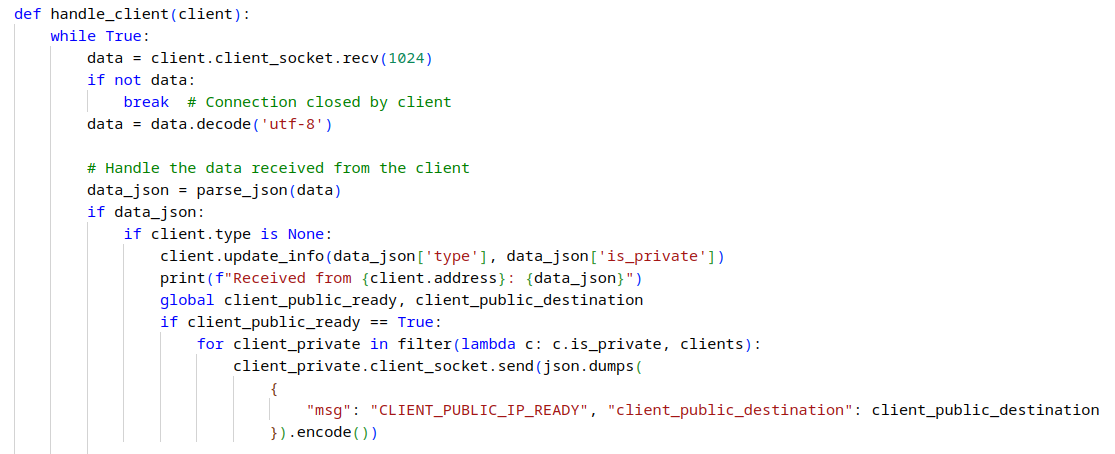
\includegraphics[width=0.8\textwidth]{gambar/kode/potongan_tracker_01}
		\caption{Potongan kode \emph{tracker} untuk klien baru terhubung}
	\end{figure}
	Setiap klien yang terhubung akan diterima oleh \emph{tracker} dan pesannya akan disimpan.

	\clearpage
	\item{Potongan kode untuk merespons \emph{manager} yang meminta kumpulan klien}
	\begin{figure}[H]
		\centering{}
		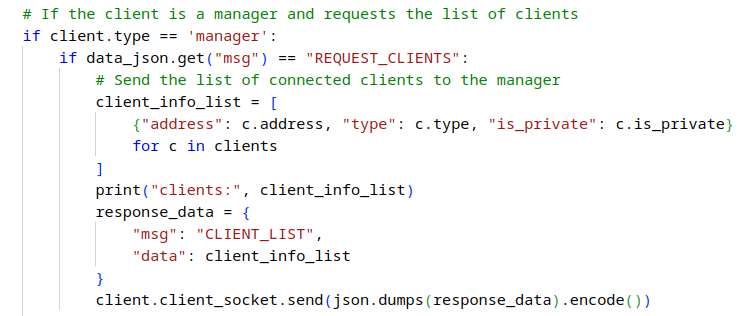
\includegraphics[width=0.8\textwidth]{gambar/kode/potongan_tracker_02}
		\caption{Potongan kode \emph{tracker} merespons \emph{manager} yang meminta kumpulan klien } 
	\end{figure}
	Setiap kali manager meminta data klien kepada \emph{tracker}. \emph{Tracker} akan merespons pesan tersebut dengan mengirim data klien kepada manager.

	\item{Potongan kode untuk merespons \emph{manager} sudah siap membuka koneksi}
	\begin{figure}[H]
		\centering{}
		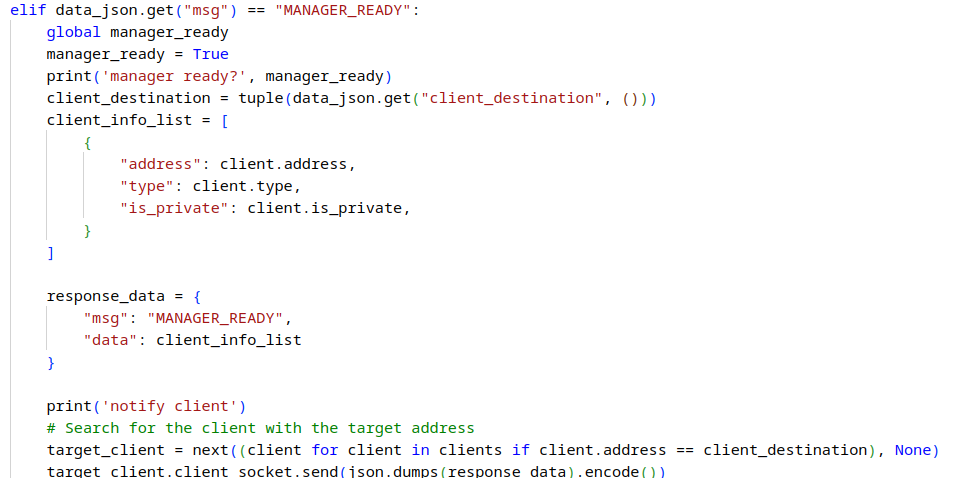
\includegraphics[width=0.8\textwidth]{gambar/kode/potongan_tracker_03}
		\caption{Potongan kode \emph{tracker} merespons \emph{manager} sudah siap membuka koneksi}
	\end{figure}
	Manager memberitahukan \emph{tracker} bahwa manager sudah siap membuka koneksi untuk dihubungkan oleh klien \emph{public}. 

	\item{Potongan kode untuk memberitahu klien \emph{private} bahwa dapat terhubung ke \emph{manager} }
	\begin{figure}[H]
		\centering{}
		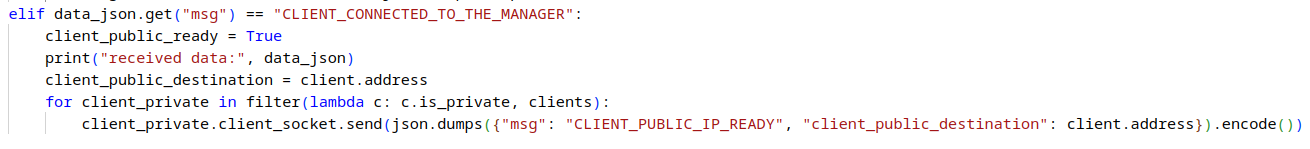
\includegraphics[width=1\textwidth]{gambar/kode/potongan_tracker_04}
		\caption{Potongan kode \emph{tracker} memberitahu klien \emph{private} untuk \emph{connect}}
	\end{figure}
	Setelah manager sudah siap untuk dihubungkan dengan klien \emph{public}. Lalu klien \emph{public} mengirimkan kembali info ke \emph{tracker} bahwa sudah terhubung ke manager, Lalu manager mengirim info ke klien \emph{private} untuk dapat terhubung ke klien \emph{public}.

\end{itemize} 

\subsection{\emph{Manager}}
\emph{Manager} akan memiliki \emph{public IP address}, dikarenakan \emph{manager} memiliki tugas untuk mengatur perangkat terhubung yang nantinya akan memiliki \emph{public IP address}. \emph{Manager} juga perlu untuk terhubung ke \emph{tracker}. \emph{Manager} mendapatkan klien yang terhubung dengan meminta data klien yang terhubung kepada \emph{tracker}. Lalu, \emph{tracker} akan mengirimkan data klien yang terhubung. \emph{Manager} akan membuka koneksi untuk klien yang nantinya memiliki \emph{public IP address} untuk terhubung dengannya.

\begin{figure}[H]
	\centering{}
	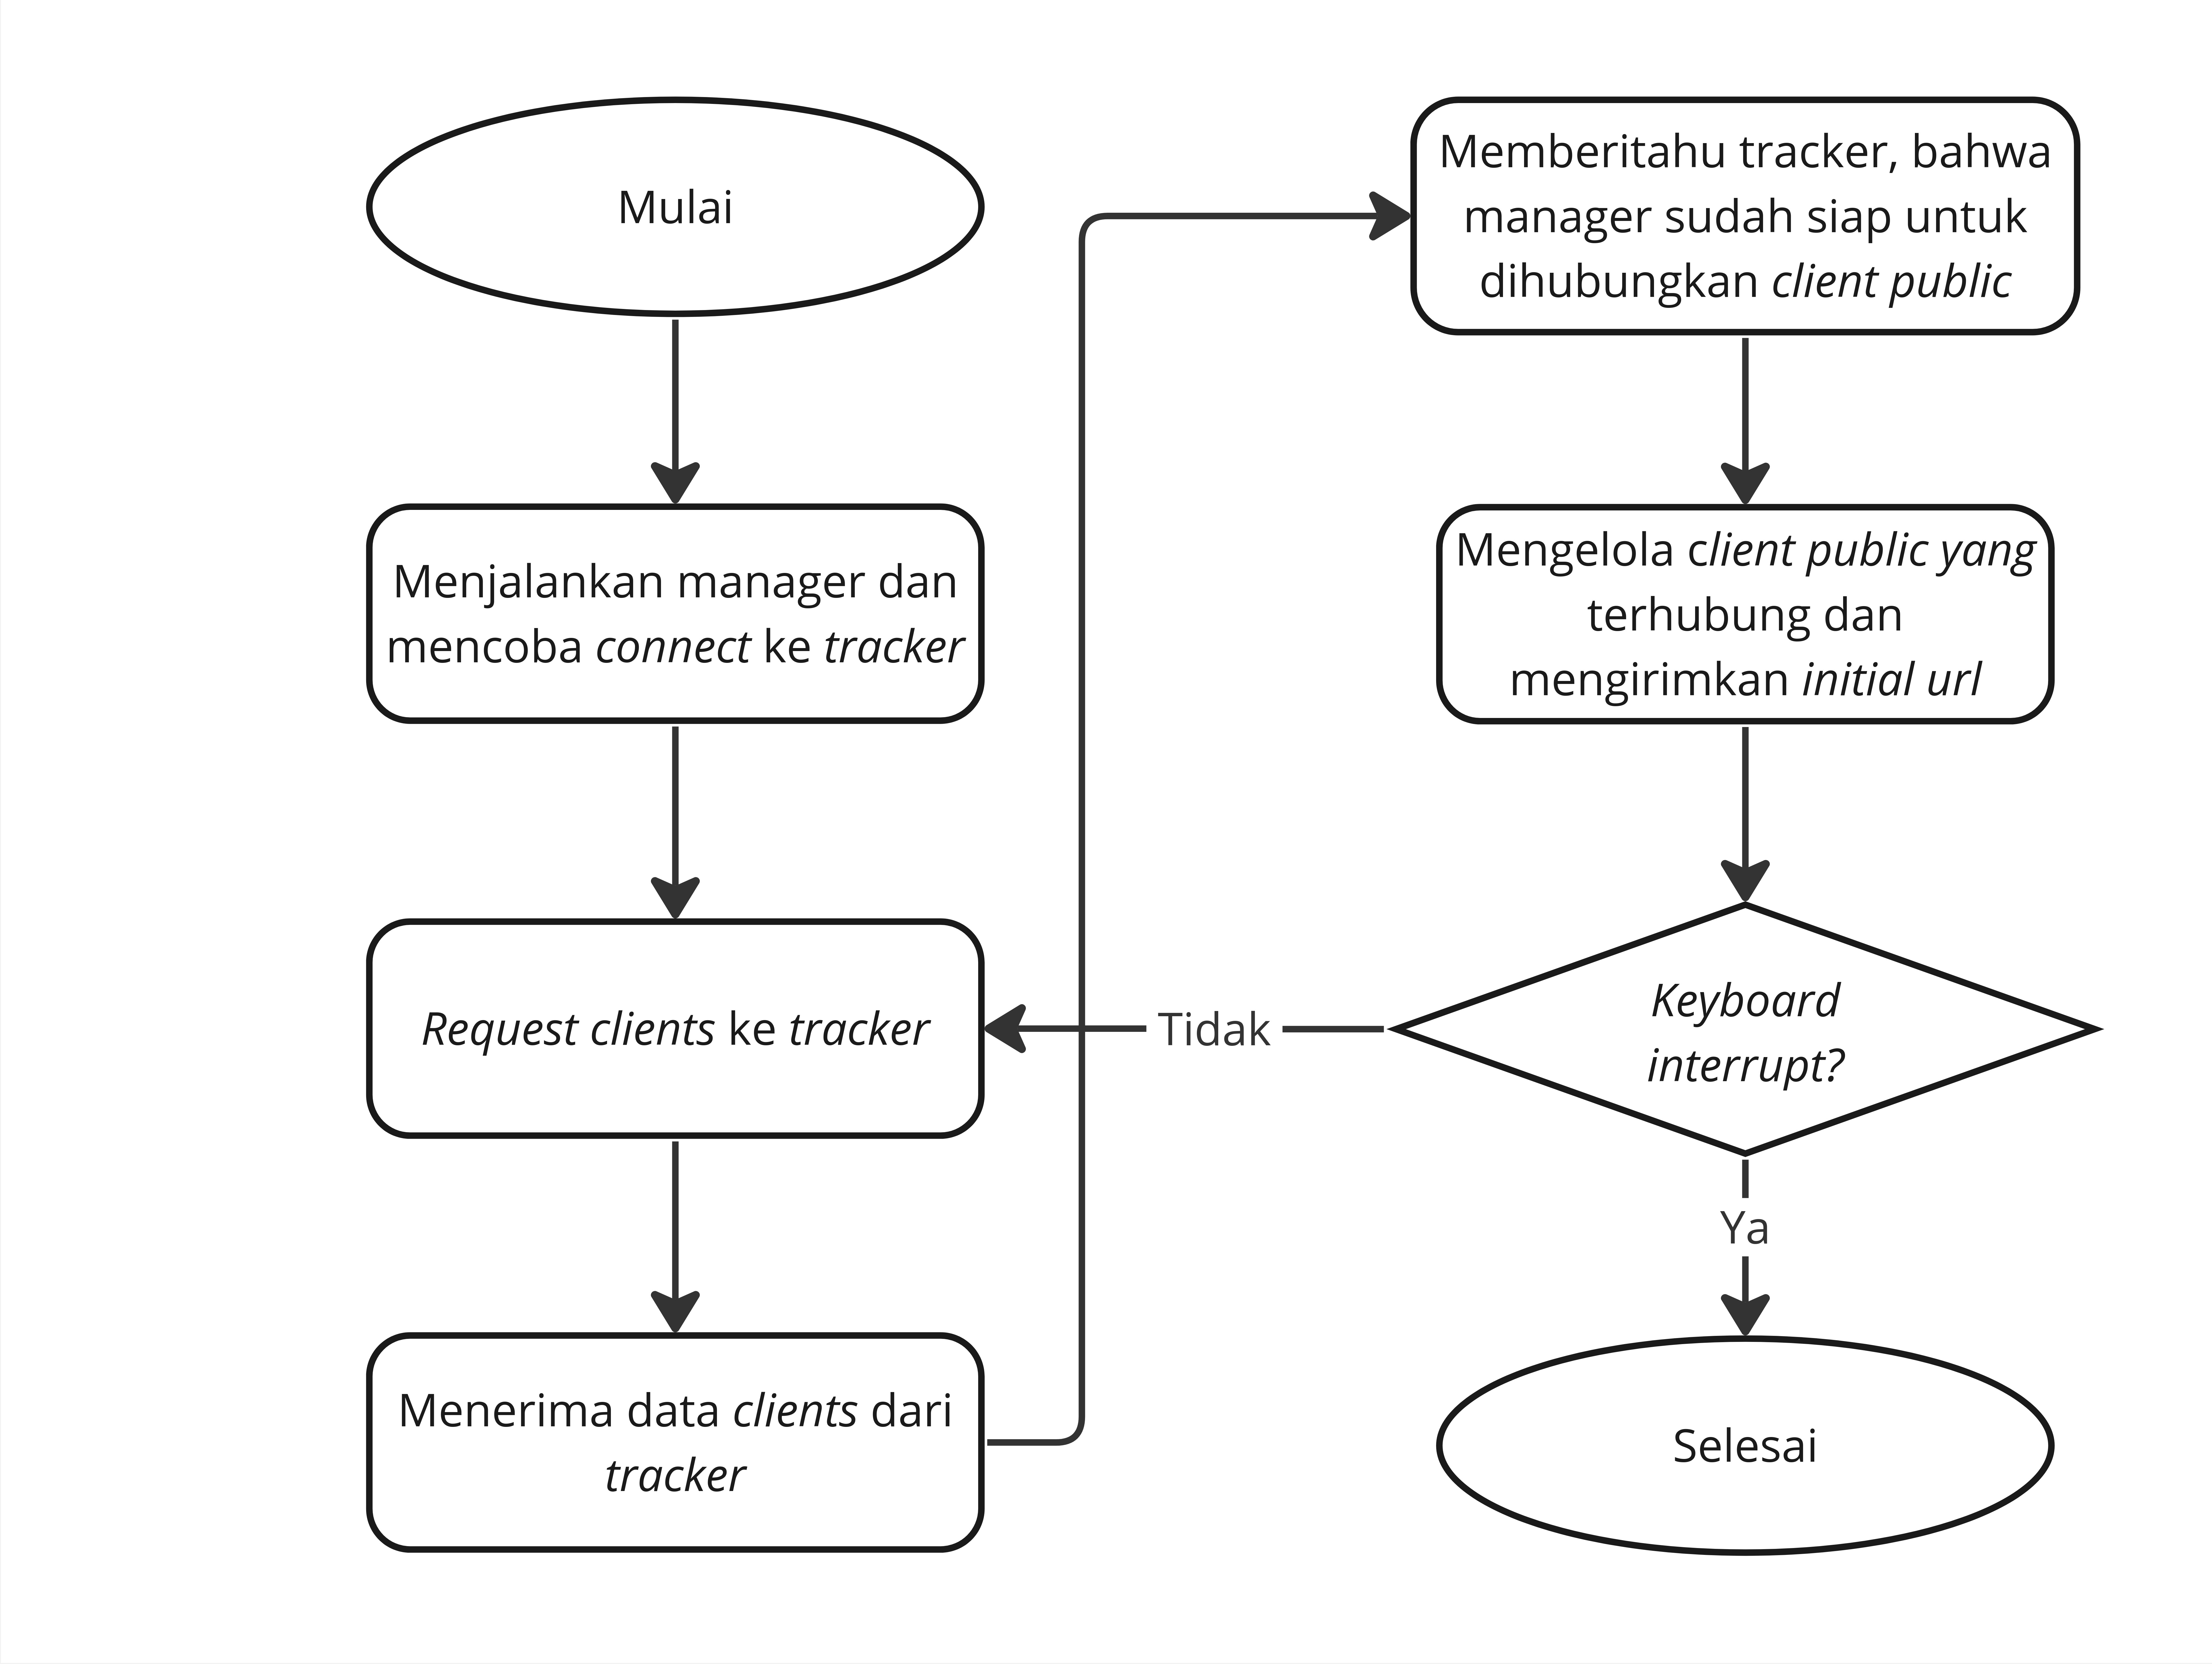
\includegraphics[width=0.8\textwidth]{gambar/flowchart_manager}
	\caption{\emph{Flowchart manager} }
\end{figure}

\begin{itemize}
	\item{Potongan kode untuk menerima kumpulan klien dari \emph{tracker} dan mengirim kembali ke \emph{tracker} bahwa \emph{manager} sudah bersedia untuk dihubungkan dengan klien \emph{public}}
	\begin{figure}[H]
		\centering{}
		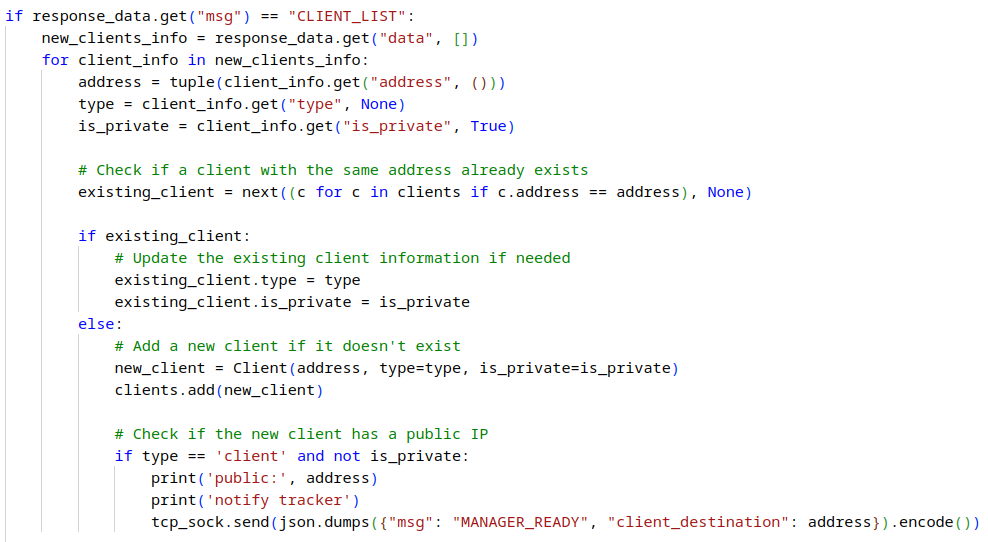
\includegraphics[width=0.8\textwidth]{gambar/kode/potongan_manager_01}
		\caption{Potongan kode \emph{manager} yang menerima data klien dan menginformasikan \emph{tracker}}
	\end{figure}

	\item{Potongan kode untuk membuka koneksi agar klien \emph{public} dapat terhubung dan inisisasi \emph{starting url}}
	\begin{figure}[H]
		\centering{}
		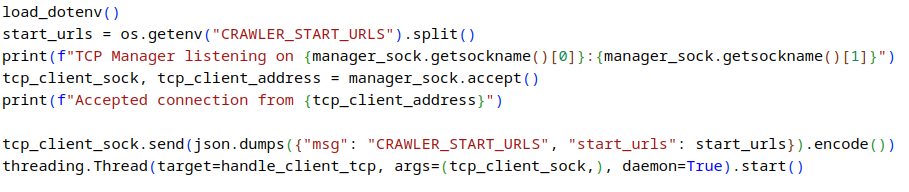
\includegraphics[width=0.8\textwidth]{gambar/kode/potongan_manager_02}
		\caption{Potongan kode \emph{manager} untuk membuka koneksi agar klien \emph{public} dapat terhubung}
	\end{figure}
\end{itemize}

\subsection{Klien}
Klien dapat memiliki \emph{public} dan \emph{private IP address}. Dalam penelitian ini terdapat 1 klien dengan \emph{public IP address} dan 2 klien dengan \emph{private IP address}, yang nantinya klien dengan \emph{private IP address} akan menjadi \emph{worker} yang melakukan \emph{crawling}. Setelah klien \emph{public} terhubung dengan \emph{tracker}. Dan \emph{tracker} juga sudah mendeteksi adanya \emph{manager} yang sudah terhubung. Maka, \emph{tracker} akan mengirim informasi \emph{manager} kepada klien tersebut. Agar klien tersebut dapat terhubung dengan \emph{manager}. Untuk klien \emph{private} nantinya akan terhubung dengan klien \emph{public} setelah mendapatkan informasi dari \emph{tracker} bahwa klien \emph{public} sudah siap untuk dihubungkan. Klien \emph{private} akan melakukan \emph{crawling} yang mana pembagian url-nya akan diatur oleh klien \emph{public}. Data hasil \emph{crawling} akan dikembalikan ke klien \emph{public} untuk disatukan. 

Proses \emph{crawling} harus dilakukan oleh klien \emph{private} dikarenakan jika dilakukan oleh klien \emph{public} akan berdampak pada \emph{Domain Name System} (DNS) klien tersebut yang dapat diblokir. Karena situs web memiliki syarat dan kebijakan yang memiliki batasan terhadap \emph{crawling} otomatis, dan dengan penggunaan klien \emph{private} dapat meminimalkan risiko. Klien \emph{private} juga membantu untuk menghindari batasan tingkat permintaan (\emph{rate limiting}), karena kalau dengan klien \emph{public} peraturannya akan lebih ketat karena terikat dari penyedia layanan internet atau server layanan.

\begin{figure}[H]
	\centering{}
	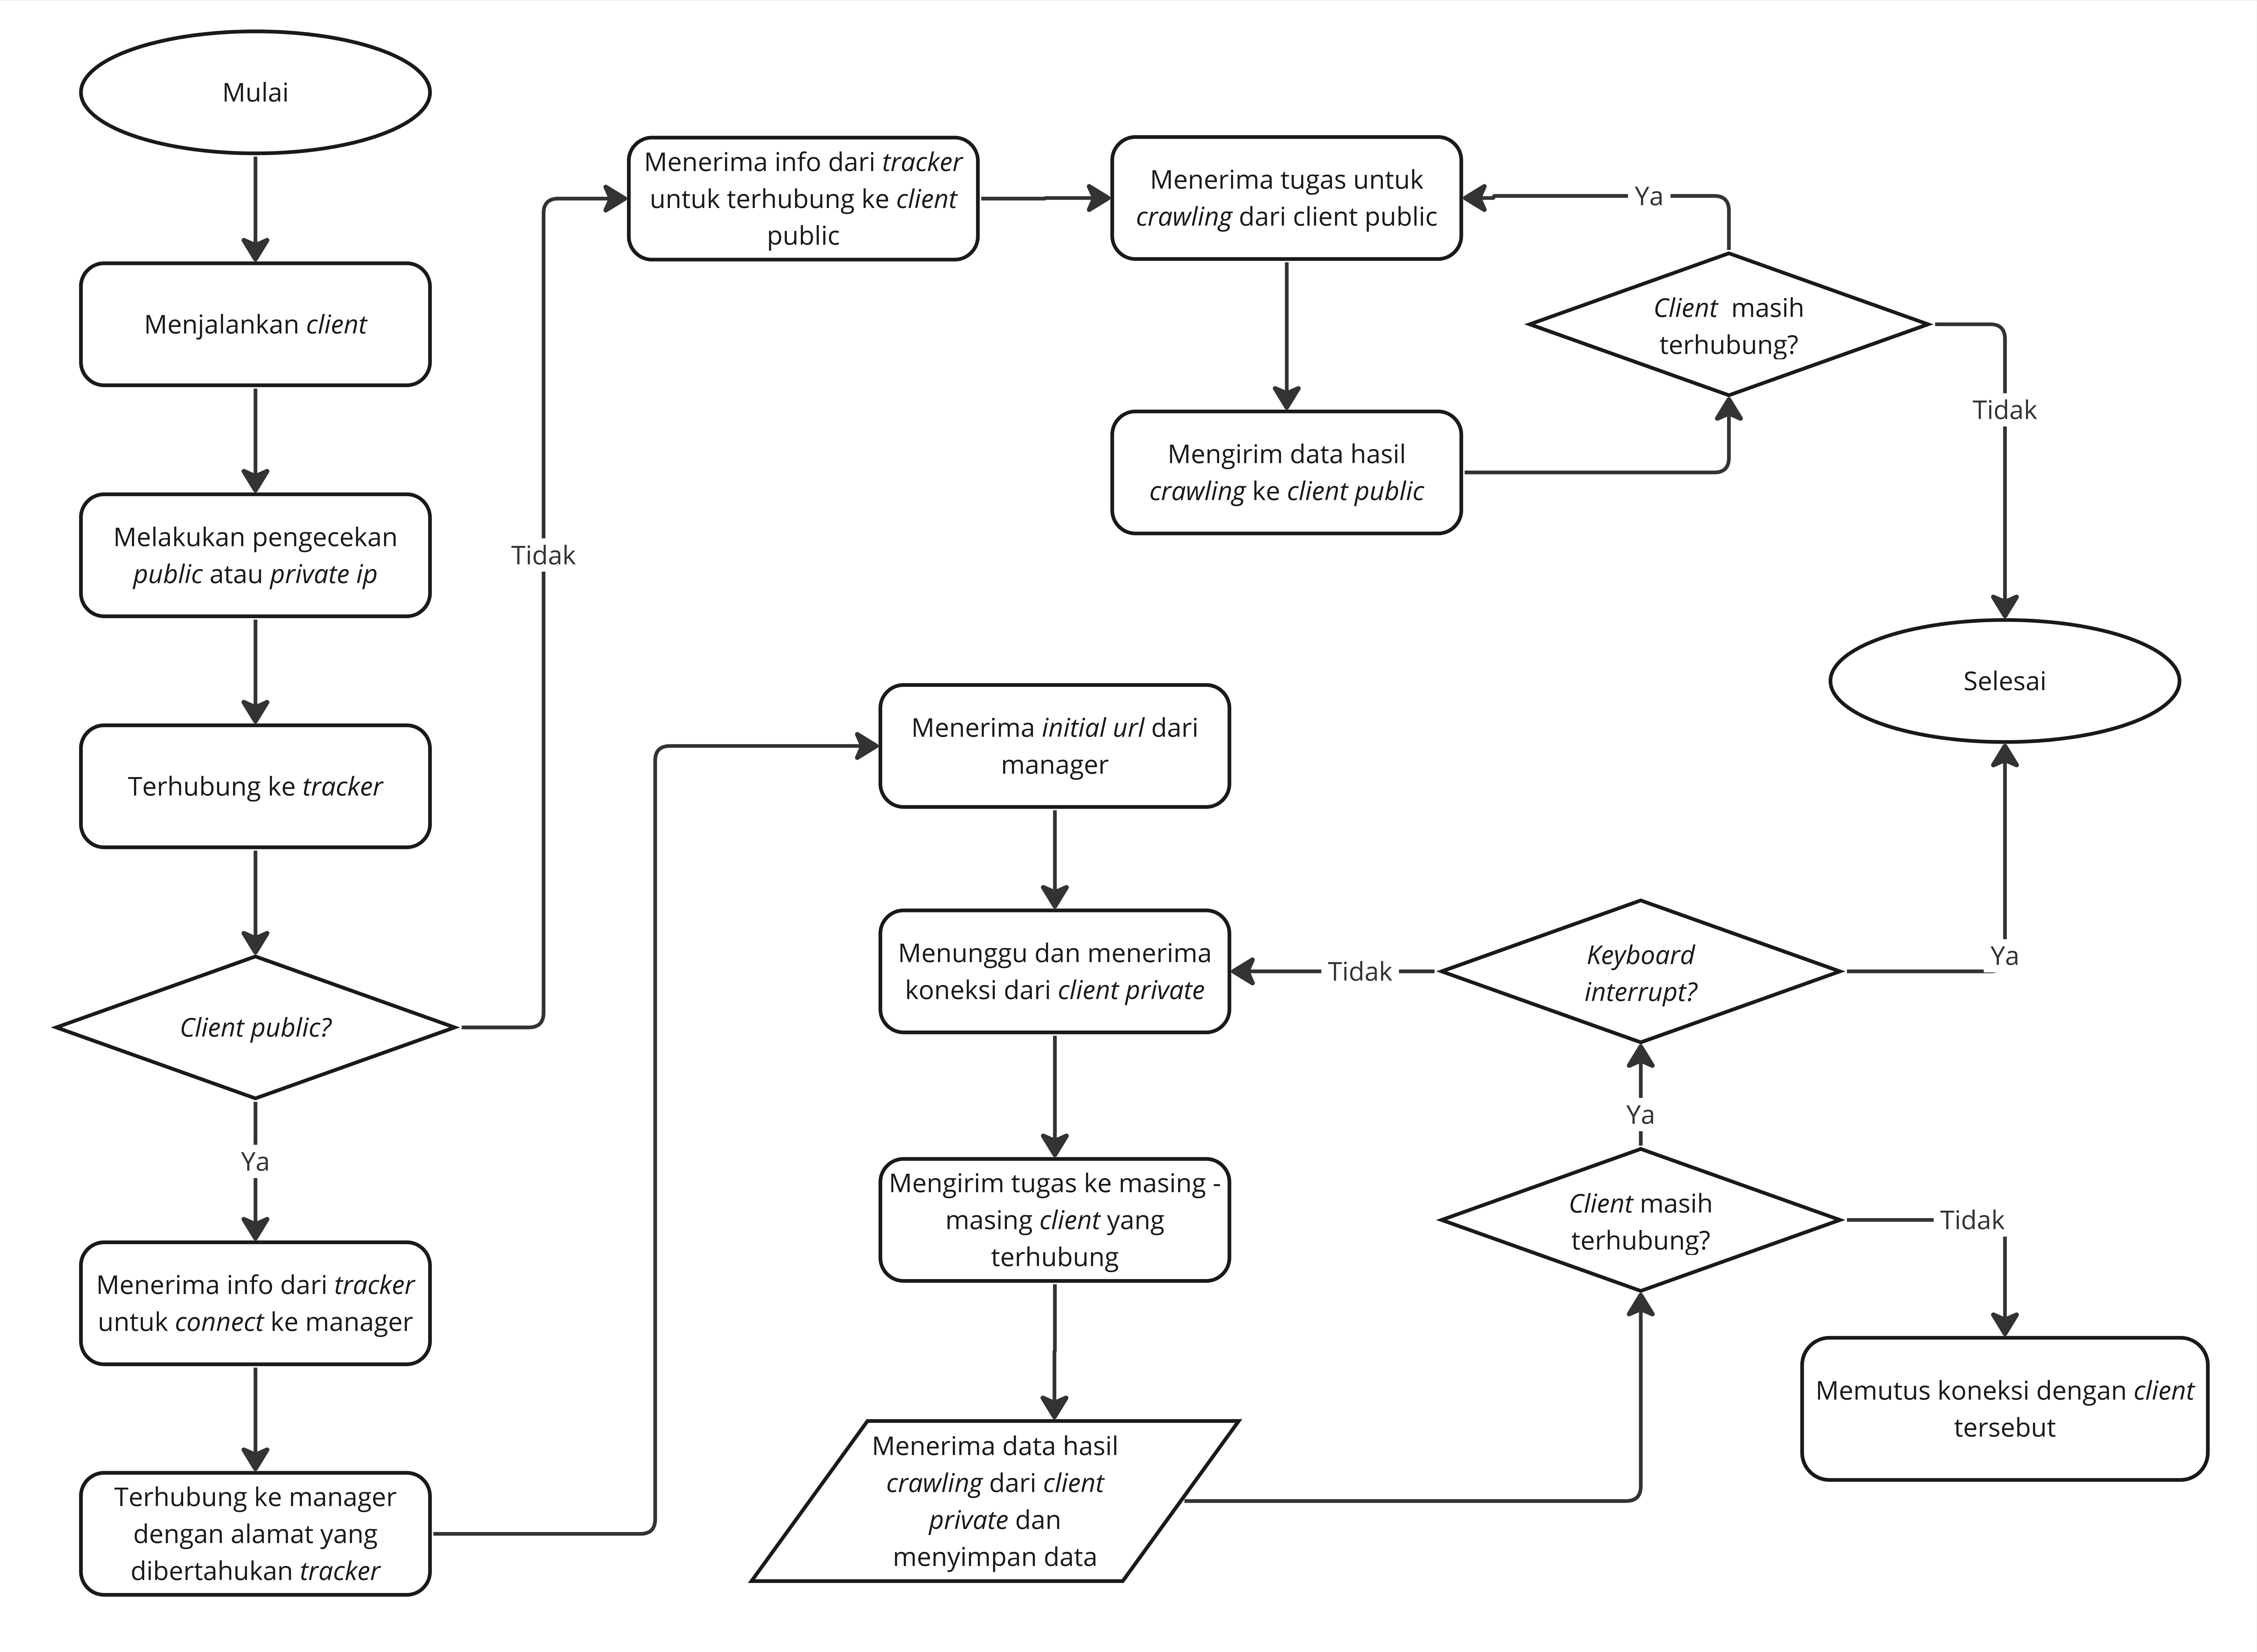
\includegraphics[width=1\textwidth]{gambar/flowchart_client}
	\caption{\emph{Flowchart client} }
\end{figure}
\clearpage

\begin{itemize}
	\item{Struktur direktori dari kode klien}
	\begin{figure}[H]
		\centering{}
		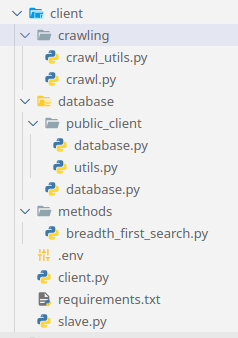
\includegraphics[width=0.4\textwidth]{gambar/kode/potongan_client_01}
		\caption{Struktur direktori kode klien}
	\end{figure}
\end{itemize}

Pada direktori \emph{"client"} terdapat tiga buah folder penunjang. \emph{"crawling"}, folder ini berisikan fungsi utama untuk melakukan \emph{crawling} serta utilitasnya. \emph{"database"}, folder ini berisikan fungsi untuk mengelola basis data, mulai dari menentukan table serta attributnya. Di folder tersebut juga terdapat \emph{"public\_client"} folder, yang berguna untuk klien \emph{public} mendefinisikan basis datanya. \emph{"methods"}, pada folder ini berisikan metode yang digunakan untuk melakukan \emph{scraping data} dari internet berdasar url yang ditentukan. 

File utama yang akan dijalankan adalah file \emph{"client.py"}. Pada file tersebut berisikan proses dari klien penentuan \emph{public} atau \emph{private} klien berdasarkan perangkat yang menjalankan program, terhubung dengan \emph{tracker}, dan melakukan komunikasi antar klien. Juga terdapat file \emph{".env"} sebagai penentuan ekosistem program, seperti berapa lamanya \emph{worker} atau klien \emph{private} akan bekerja. File \emph{"requirements.txt"} berisikan modul - modul yang diperlukan untuk menjalankan program. File \emph{"slave.py"} juga tidak kalah penting, karena didalamnya terdapat fungsi - fungsi untuk membantu pengiriman data ke klien \emph{public}. Pada penelitian ini akan lebih mendalam membahas tentang proses distribusinya. Karena untuk metode \emph{crawling} sebagian besar akan sama dengan penelitian terdahulu (\cite{lazuardy2023search}).
\clearpage

\begin{itemize}
	\item{Fungsi untuk mendapatkan IP \emph{address} apakah \emph{public} atau \emph{private}}
	\begin{figure}[H]
		\centering{}
		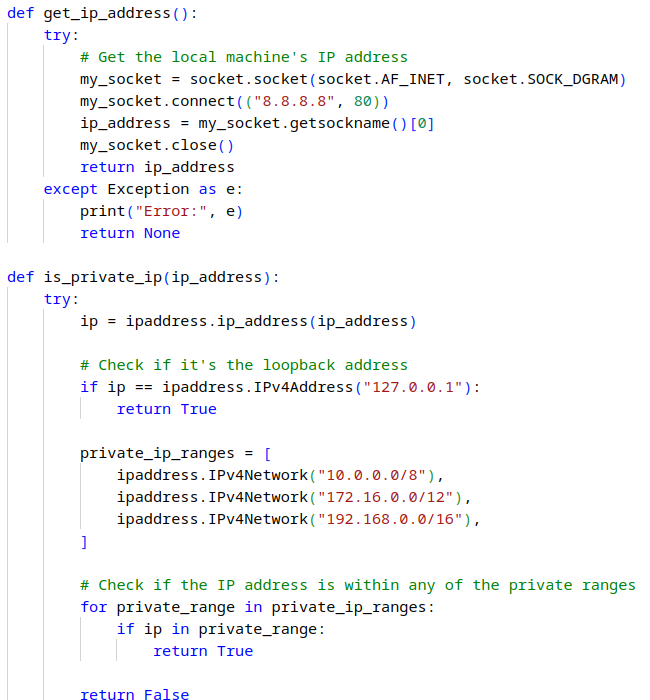
\includegraphics[width=1\textwidth]{gambar/kode/potongan_client_00}
		\caption{Fungsi untuk mendapatkan IP \emph{address} apakah \emph{public} atau \emph{private}}
	\end{figure}
\end{itemize}
Pada fungsi ini dapat menentukan IP \emph{address}-nya dengan cara mendapatkan \emph{socket address} yang sudah terhubung dengan \emph{socket} lain. Dan \emph{address}-nya akan dibandingkan dengan IP address \emph{private}. Kalau tidak sama, berarti \emph{address} tersebut adalah \emph{public}. Kalau sama, berarti \emph{private}. 

\clearpage
\subsubsection{Klien \emph{Public}}

\begin{itemize}
	\item{Pendeklarasian kelas \emph{Client}}
	\begin{figure}[H]
		\centering{}
		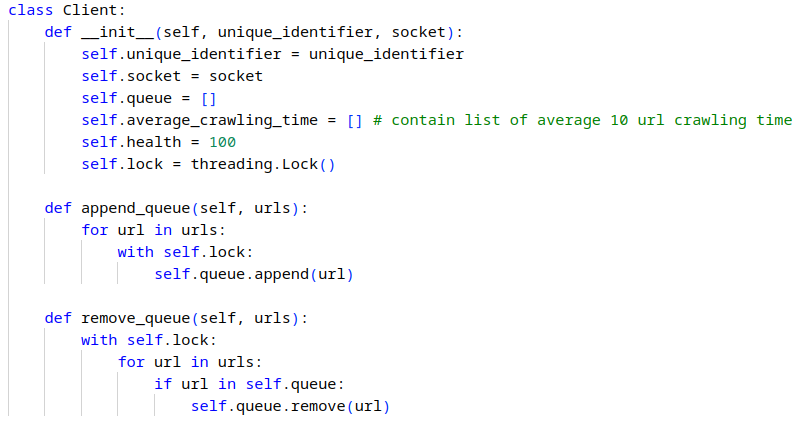
\includegraphics[width=1\textwidth]{gambar/kode/potongan_client_02}
		\caption{Pendeklarasian kelas \emph{Client}}
	\end{figure}

	\item{Pendeklarasian kelas \emph{LoadBalancer}}
	\begin{figure}[H]
		\centering{}
		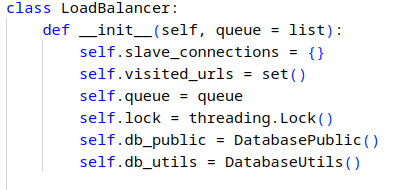
\includegraphics[width=0.8\textwidth]{gambar/kode/potongan_client_03}
		\caption{Pendeklarasian kelas \emph{LoadBalancer}}
	\end{figure}

	\clearpage
	\item{Potongan kode \emph{public} untuk merespons komunikasi dengan \emph{tracker} untuk mendapatkan informasi ketika \emph{manager ready} dan menginformasikan klien \emph{private} untuk terhubung}
	\begin{figure}[H]
		\centering{}
		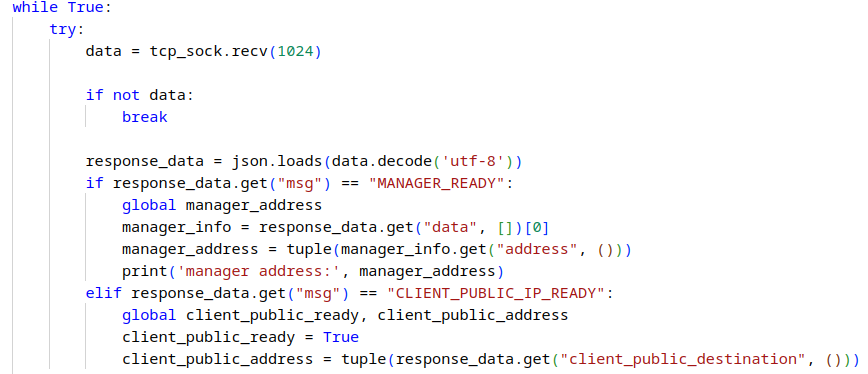
\includegraphics[width=1\textwidth]{gambar/kode/potongan_client_09}
		\caption{Potongan kode klien \emph{private}}
	\end{figure}

	\item{Potongan kode klien \emph{public} mencoba terhubung dengan \emph{manager}}
	\begin{figure}[H]
		\centering{}
		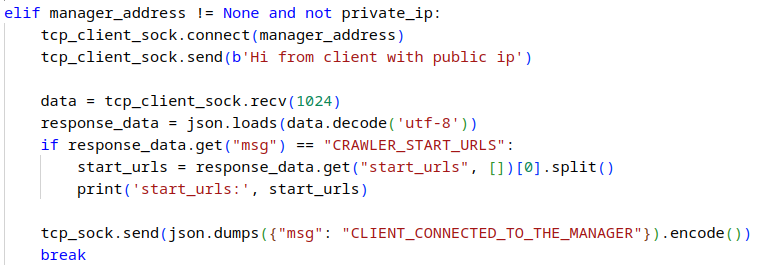
\includegraphics[width=1\textwidth]{gambar/kode/potongan_client_10}
		\caption{Potongan kode klien \emph{public} mencoba terhubung dengan \emph{manager}}
	\end{figure}
	\clearpage

	\item{Potongan kode komunikasi antar klien serta mengirimkan url pertama untuk di-\emph{crawling} kepada klien \emph{private}}
	\begin{figure}[H]
		\centering{}
		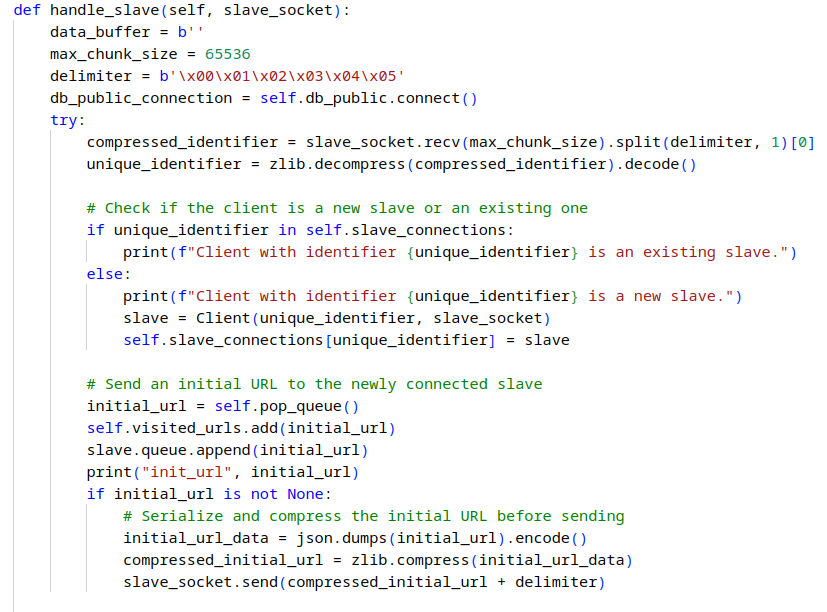
\includegraphics[width=1\textwidth]{gambar/kode/potongan_client_04}
		\caption{Potongan kode komunikasi antar klien}
	\end{figure}
	Klien \emph{public} akan mengatur klien \emph{private} yang terhubung. Menyimpan \emph{unique identifier}-nya, akan dipastikan bahwa tidak ada klien \emph{private} dengan address yang sama terhubung. Dan tentunya akan menghapus klien \emph{private} yang sudah tidak lagi terhubung lagi dengan klien \emph{public}. Pencatatan jumlah url untuk setiap klien \emph{private} juga dipertimbangkan.
	
	Serta pengiriman data akan di-\emph{encode} ke JSON dan di-\emph{compress} agar data yang dikirimkan tidak begitu besar. Setiap data yang diterima oleh klien \emph{public} pun juga akan di-\emph{decompress}. 

	\item{Potongan kode klien \emph{public} menerima data hasil \emph{crawling} yang diberikan oleh klien \emph{private} serta memasukkan informasi terkait ke dalam database}
	\begin{figure}[H]
		\centering{}
		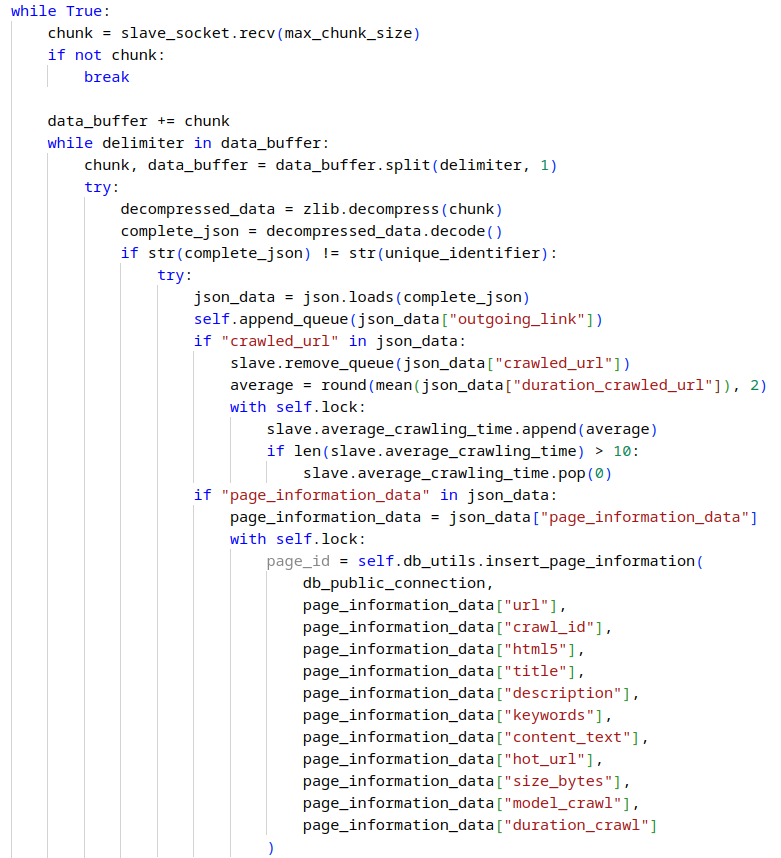
\includegraphics[width=0.8\textwidth]{gambar/kode/potongan_client_05}
		\caption{Potongan kode klien \emph{public} menerima data hasil \emph{crawling}}
	\end{figure}

	\item{Fungsi untuk pengecekan duplikasi url yang didapatkan dari hasil \emph{crawling}}
	\begin{figure}[H]
		\centering{}
		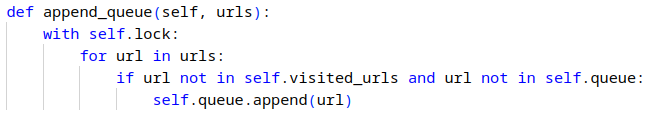
\includegraphics[width=1\textwidth]{gambar/kode/potongan_client_06}
		\caption{Fungsi untuk pengecekan duplikasi url yang didapatkan dari hasil \emph{crawling}}
	\end{figure}

	\item{Potongan kode klien \emph{public} mengirimkan url yang akan di-\emph{crawling} ke klien \emph{private} dengan mempertimbangkan kondisi dari klien tersebut berdasarkan kecepatan \emph{crawling}. Klien yang lambat akan dikirim sedikit url untuk mengurangi bebannya. Sedangkan, klien yang cepat akan mendapatkan jumlah tugas lebih banyak.}

	\begin{figure}[H]
		\centering{}
		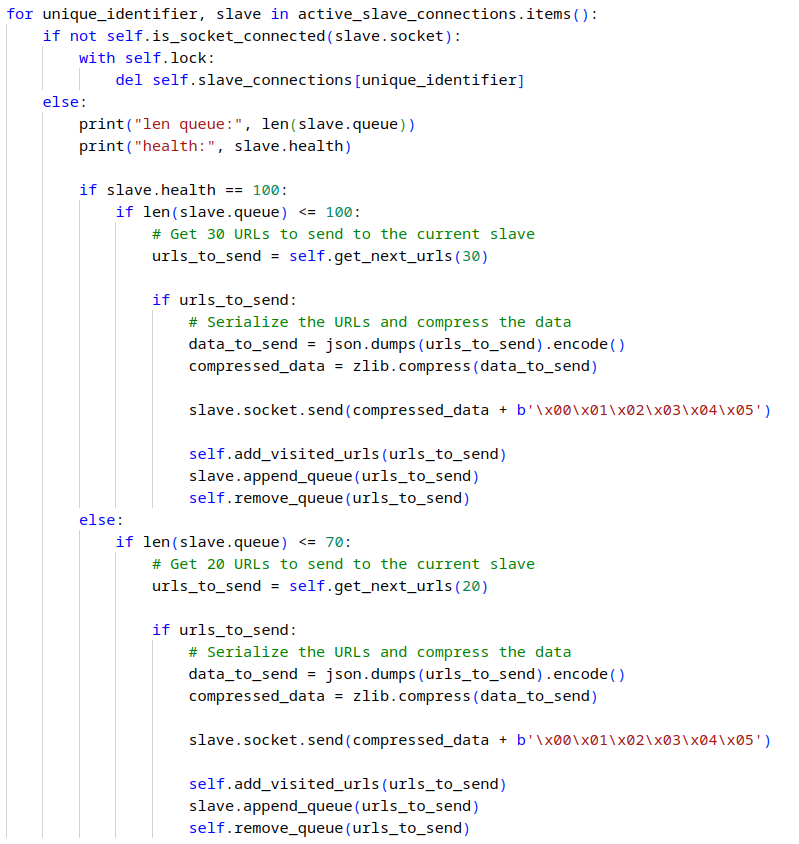
\includegraphics[width=1\textwidth]{gambar/kode/potongan_client_07}
		\caption{Potongan kode klien \emph{public} mengirimkan url yang akan di-\emph{crawling}}
	\end{figure}
	Setiap beberapa detik sekali klien \emph{public} akan mengirimkan url yang akan di-\emph{crawling} oleh klien \emph{private}. Url yang dikirim sudah dipastikan tidak terduplikasi dan dilakukan \emph{compress}. Penentuan pengiriman jumlah url juga ditentukan dari "kesehatan" dari klien \emph{private}. Kalau kondisinya "sehat", maka akan mendapatkan 30 url setiap kiriman dan sebaliknya akan mendapatkan 20 url.

	\clearpage
	\item{Fungsi untuk pengecekan "kesehatan" dari setiap klien yang terhubung}
	\begin{figure}[H]
		\centering{}
		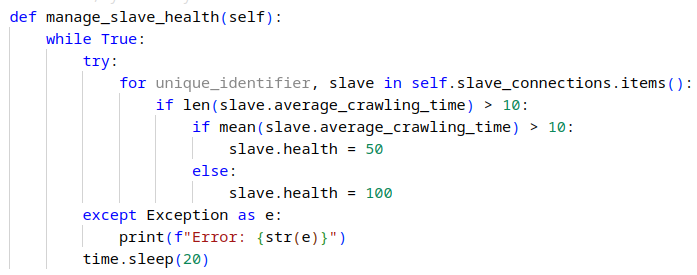
\includegraphics[width=1\textwidth]{gambar/kode/potongan_client_08}
		\caption{Fungsi untuk pengecekan "kesehatan" dari setiap klien yang terhubung}
	\end{figure}
\end{itemize}

\subsubsection{Klien \emph{Private}}

\begin{itemize}
	\item{Fungsi untuk klien \emph{private} terhubung ke klien \emph{public}}
	\begin{figure}[H]
		\centering{}
		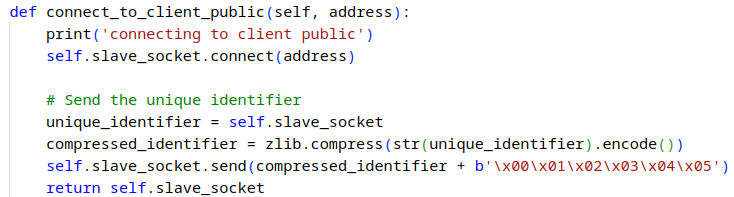
\includegraphics[width=1\textwidth]{gambar/kode/potongan_client_11}
		\caption{Fungsi untuk klien \emph{private} terhubung ke klien \emph{public}}
	\end{figure}
	Ketika pertama kali klien \emph{private} terhubung ke klien \emph{public}. Maka akan mengirimkan \emph{unique identifier} untuk membedakan client yang terhubung. Dan tidak lupa pula untuk di-\emph{compress}.

	\clearpage
	\item{Fungsi untuk klien \emph{private} menerima url yang akan di-\emph{crawling} dari klien \emph{public}}
	\begin{figure}[H]
		\centering{}
		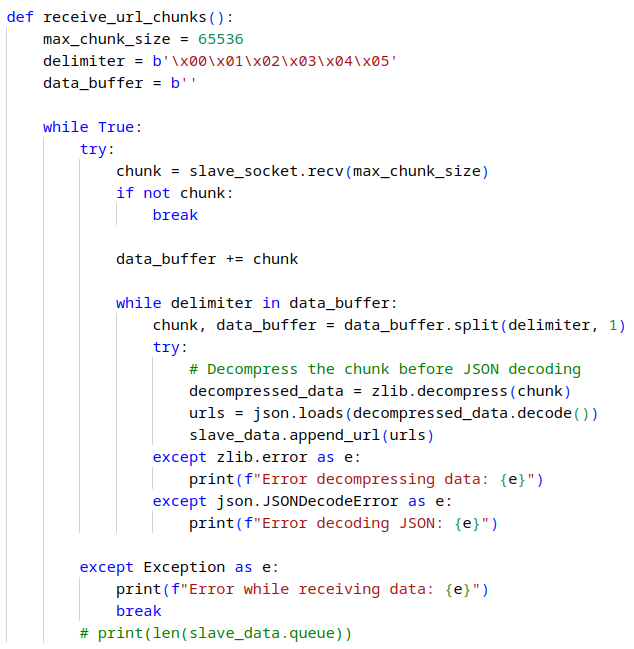
\includegraphics[width=1\textwidth]{gambar/kode/potongan_client_12}
		\caption{Fungsi untuk klien \emph{private} menerima url yang akan di-\emph{crawling} dari klien \emph{public}}
	\end{figure}

	\clearpage
	\item{Potongan kode dari fungsi untuk klien \emph{private} mengirim url hasil \emph{crawling} ke klien \emph{public}}
	\begin{figure}[H]
		\centering{}
		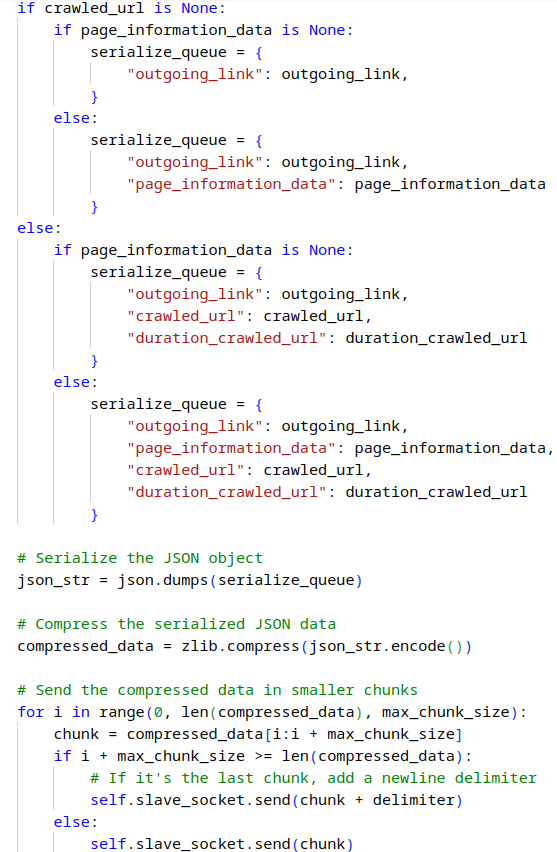
\includegraphics[width=0.8\textwidth]{gambar/kode/potongan_client_13}
		\caption{Potongan kode dari fungsi untuk klien \emph{private} mengirim url hasil \emph{crawling} ke klien \emph{public}}
	\end{figure}

	\clearpage
	\item{Potongan kode dari fungsi untuk klien \emph{private} melakukan \emph{scraping} halaman web}
	\begin{figure}[H]
		\centering{}
		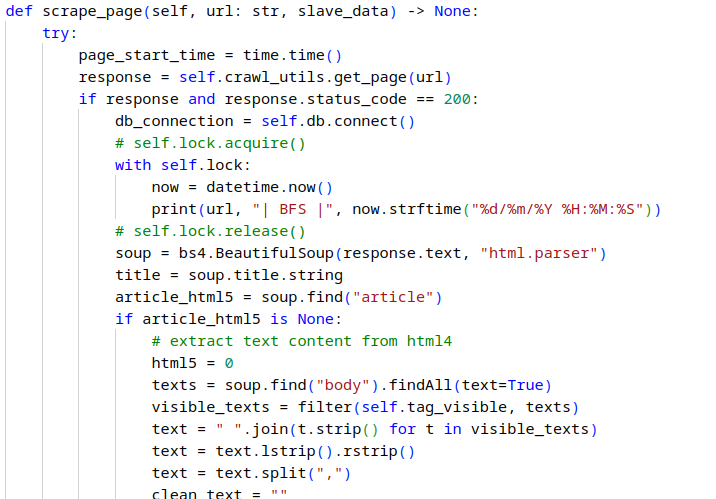
\includegraphics[width=1\textwidth]{gambar/kode/potongan_client_14}
		\caption{Potongan kode untuk klien \emph{private} melakukan \emph{scraping} halaman web}
	\end{figure}
\end{itemize}

\section{Pengujian}

Pada penelitian ini akan terfokus untuk menguji proses komunikasi yang terjadi, konsistensi data, efisiensi sumber daya dan optimalisasi data . Dijalankan proses \emph{crawling} selama satu jam. Pada \emph{crawler} individual dan \emph{crawler} terdistribusi. Pengujian dilakukan dengan \emph{initial url}: "https://www.detik.com/". 


\begin{table}[H]
	\begin{center}
		\caption{\label{tabel:hasil_crawling} Hasil \textit{crawling} selama satu jam}
		\begin{tabular}{|c|c|c|} 
			\hline
				Jenis \textit{Crawler} & \textit{Total Rows} & \textit{Unique Rows} \\ 
			\hline
				\textit{Crawler} Individual & 7069 & 7069 \\
			\hline
				2 \textit{Crawler} Terdistribusi & 9175 & 9175 \\
			\hline
		\end{tabular}
	\end{center}
\end{table}

% \begin{figure}[H]
% 	\centering{}
% 	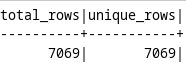
\includegraphics[width=0.4\textwidth]{gambar/hasil/hasil_satu_jam_crawler_individual}
% 	\caption{Hasil dari \emph{crawling} dengan \emph{crawler} individual selama satu jam}
% \end{figure}

% \begin{figure}[H]
% 	\centering{}
% 	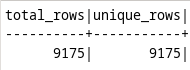
\includegraphics[width=0.4\textwidth]{gambar/hasil/hasil_satu_jam_crawler_terdistribusi_dua_crawler}
% 	\caption{Hasil dari \emph{crawling} dengan \emph{crawler} terdistribusi selama satu jam dengan skema dua \emph{crawler}}
% \end{figure}

\subsection{Proses Komunikasi}
Berikut adalah proses komunikasi pada setiap perangkat:
\begin{itemize}
	\item{Proses komunikasi pada \emph{tracker}}
	\begin{figure}[H]
		\centering{}
		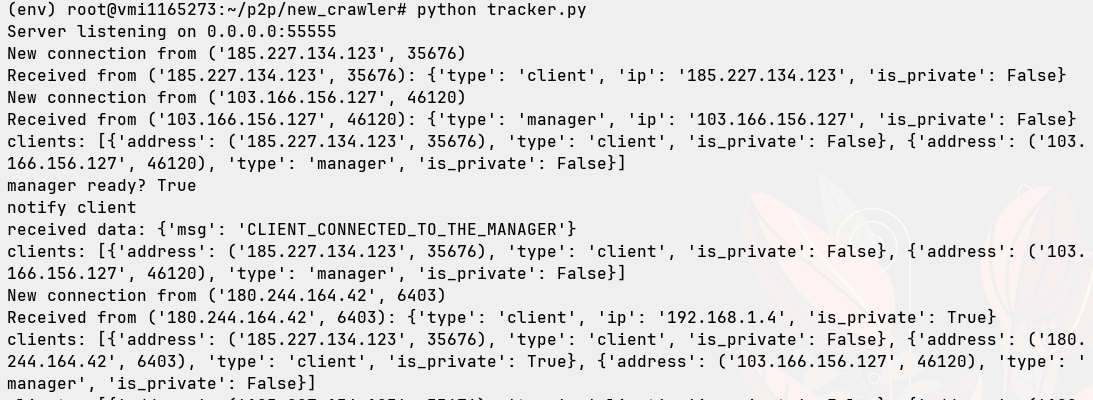
\includegraphics[width=0.8\textwidth]{gambar/kode/uji_tracker}
		\caption{Proses komunikasi pada \emph{tracker}}
	\end{figure}

	\item{Proses komunikasi pada \emph{manager}}
	\begin{figure}[H]
		\centering{}
		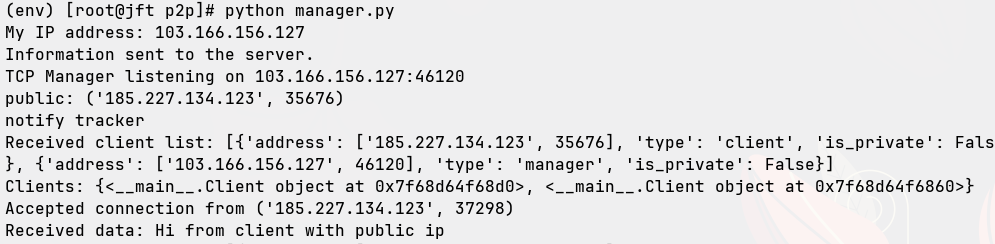
\includegraphics[width=0.8\textwidth]{gambar/kode/uji_manager}
		\caption{Proses komunikasi pada \emph{manager}}
	\end{figure}

	\item{Proses komunikasi pada klien \emph{public}}
	\begin{figure}[H]
		\centering{}
		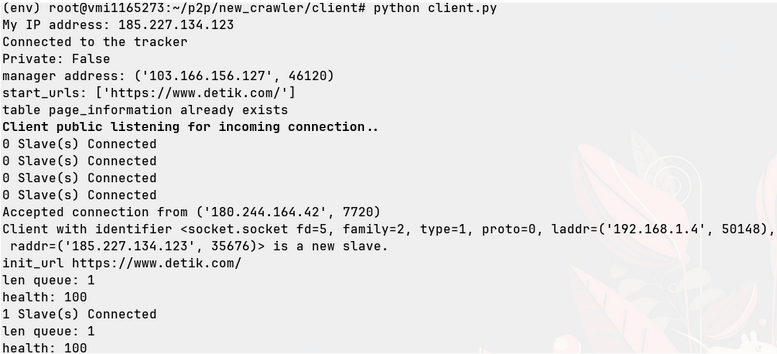
\includegraphics[width=0.8\textwidth]{gambar/kode/uji_client_public}
		\caption{Proses komunikasi pada klien \emph{public}}
	\end{figure}

	\item{Proses komunikasi pada klien \emph{private}}
	\begin{figure}[H]
		\centering{}
		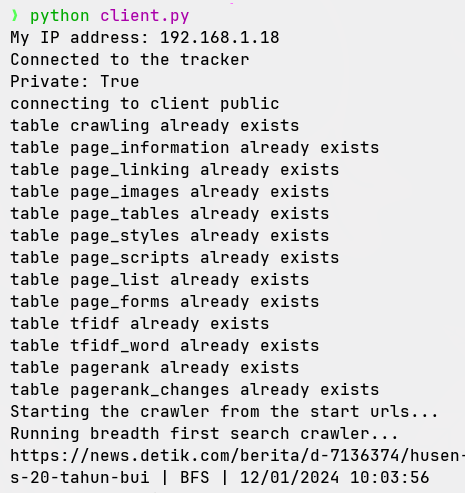
\includegraphics[width=0.6\textwidth]{gambar/kode/uji_client_private}
		\caption{Proses komunikasi pada klien \emph{private}}
	\end{figure}
\end{itemize}

\subsection{Konsistensi Data}
Berdasarkan Tabel 4.1, didapatkan hasil data url yang di-\emph{crawling} itu unik dan tidak ada duplikasi. Berdasarkan hasil perhitungan sebagai berikut.
\[
\text{Jumlah baris yang terduplikasi} = \emph{Total Rows} - \emph{Unique Rows} = 9175 - 9175 = 0
\]

\subsection{Efisien Sumber Daya dan Optimalisasi Data}
Berdasarkan Tabel 4.1, didapatkan hasil peningkatan jumlah data dengan waktu yang relatif sama, yaitu satu jam. Pada \emph{crawler} individual didapatkan jumlah baris data dalam tabel database sebanyak 7069 dan pada \emph{crawler} terdistribusi didapatkan jumlah baris data dalam tabel database sebanyak 9175. Terdapat peningkatan jumlah data yang didapatkan oleh \emph{crawler} terdistribusi. Penambahan total data yang terkumpul dapat dicapai beriringan dengan sumber daya yang digunakan secara efisien.

$\text{Persentase peningkatan data} = \left( \frac{9175 - 7069}{7069} \right) \times 100 \approx 30.0\%$

\section{Analisis Hasil}
Berdasarkan proses perbandingan \emph{crawling} yang berjalan selama satu jam, analisis hasil pengujian adalah sebagai berikut:

\begin{enumerate}
	\item Proses komunikasi antar perangkat berjalan dengan sistematis.

	\item Data yang dihasilkan dari \emph{crawler} terdistribusi lebih banyak daripada \emph{crawler} individual. Didapatkan sekitar 30\% lebih banyak.
	
	\item Duplikasi data dapat terhindarkan saat mengelola lebih dari satu \emph{crawler} dengan melakukan \emph{crawling} berdasarkan url yang diterima dari pengelola (klien \emph{public}) dan mengembalikan temuan url baru kepada pengelola.

	\item Efisiensi sumber daya dan optimalisasi data dapat tercapai, hanya dengan melakukan \emph{crawling} selama satu jam. Bisa lebih dari satu \emph{crawler} yang berjalan di satu waktu yang bersamaan. Peningkatan tersebut juga dipengaruhi oleh latensi jaringan, \emph{overhead} koordinasi, dan potensi \emph{bottleneck}.

	\item Proses penyatuan data menjadi \emph{centralized} pada satu perangkat, yang mana merupakan penggabungan dari setiap \emph{crawler} yang melakukan pekerjaan.
\end{enumerate}

Hasil perbandingan \emph{crawler} individual dengan \emph{crawler} terdistribusi menunjukkan hasil yang baik. Peningkatan efisiensi dapat diraih dengan menerapkan metode terdistribusi. Ada hal yang harus dibayar dalam meningkatkan efisiensi, walaupun perbedaan yang terlihat hanya 30\% tapi itu merupakan hal yang baik karena hasil akhirnya mengalami peningkatan. 

% Baris ini digunakan untuk membantu dalam melakukan sitasi
% Karena diapit dengan comment, maka baris ini akan diabaikan
% oleh compiler LaTeX.
\begin{comment}
\bibliography{daftar-pustaka}
\end{comment}
